\documentclass[a4paper]{report}
\usepackage{inputenc}
\usepackage[T1]{fontenc}
\usepackage{RJournal}
\usepackage{amsmath,amssymb,array}
\usepackage{booktabs}
\usepackage[ruled,vlined]{algorithm2e}
\usepackage{nicefrac}
%\usepackage{verbatimbox}

\DeclareMathOperator*{\argmin}{arg\,min}
\DeclareMathOperator*{\argmax}{arg\,max}

\newcommand{\minsestelo}{\operatornamewithlimits{min}}

%% load any required packages here

\begin{document}

%% do not edit, for illustration only
\sectionhead{Contributed research article}
\volume{13}
\volnumber{1}
\year{2021}
\month{June}
\setcounter{page}{164}

%% replace RJtemplate with your article
\begin{article}
  %
% *****************************************
% This file is defunct: for R Journal files please visit:
% https://journal.r-project.org/
% *****************************************

\title{\pkg{clustcurv}: An R Package for Determining Groups in Multiple Curves }
\author{by Nora M. Villanueva, Marta Sestelo, Luis Meira-Machado and Javier Roca-Pardi\~nas} 

\maketitle

\abstract{ 
In many situations, it could be interesting to ascertain whether groups of curves can be performed, especially when confronted with a considerable number of curves. This paper introduces an R package, known as \CRANpkg{clustcurv}, for determining clusters of curves with an automatic selection of their number. The package can be used for determining groups in multiple survival curves as well as for multiple regression curves. Moreover, it can be used with large numbers of curves. An illustration of the use of \pkg{clustcurv} is provided, using both real data examples and artificial data. 
}

\noindent \textit{Keywords}: multiple curves, number of groups, nonparametric, survival analysis, regression models, cluster


\section{Introduction}
\label{intro}

A problem often encountered in many fields is the comparison of several populations through specific curves. Typical examples, considered by a number of authors, are given by the comparison of survival curves in survival analysis, children growth curves in pediatrics, or the comparison of regression curves in regression analysis.  In many of these studies, it is very common to compare a large number of curves between groups, and methods of summarizing and extracting relevant information are necessary. A common approach is to look for a partition of the sample into a number of groups in such a way that curves in the same group are as alike as possible but as distinct as possible from those in other groups. This process is also known as curve clustering. A hypothesis test can be used to ascertain that the curves in the same group are equal. A fundamental and difficult problem in clustering curves is the estimation of the number of clusters in a dataset.


Traditionally, the comparison of these functions is performed using parametric models through the comparison of the resulting model parameters. This approach, however, requires the specification of the parametric model, which is often difficult and may be considered a disadvantage. Several nonparametric methods have been proposed in the literature to compare multiple curves. In the area of survival analysis, for example, several nonparametric methods have been proposed to test for the equality of survival curves for censored data. The most well-known and widely used to test the null hypothesis of no difference in survival between two or more independent groups was proposed by \citet{mantel}. An alternative test that is often used is the Peto \& Peto \citep{CIS-11103} modification of the Gehan-Wilcoxon test \citep{10.2307/2333825}.  Several other variations of the log-rank test statistic using weights on each event time have been proposed in the literature \citep{CIS-23788,doi:10.1093/biomet/69.3.553,10.2307/2289169} as well as other procedures to compare these survival curves based on different measures, as can be the medians \citep{Chen2016}. There exists an extensive literature on curve comparison in the framework of regression analysis. In this context, several nonparametric tests have been proposed to test the equality of the mean functions, $H_0:m_1=\cdot \cdot \cdot =m_j$. \citet{hall1990}  proposed a bootstrap test, while \citet{hardle} Hardle and Marron (1990) suggested a semiparametric approach based on kernel smoothing. Other relevant papers on this topic are  \citet{king91} , \citet{Delgado} , \citet{kulasekera95} , \citet{bowman95}, \citet{dette2001}, \citet{Pardo} , \citet{Srihera:2010:NCR:1837522.1837642} , among others. A good review on this topic can be seen in the paper by \citet{neumeyer03}.

When the null hypothesis of equality of curves is rejected, leading to the clear conclusion that at least one curve is different, it can be interesting to ascertain whether curves can be grouped or if all these curves are different from each other. In this setting, one naïve approach would be to perform pairwise comparisons. In this line are the papers by \citet{Rosenblatt1975}, \citet{cao}, \citet{hardle}, \citet{dette2001} who proposed alternative tests of the null hypothesis of equality of curves obtained from pairwise comparisons of the estimators of the regression functions. A similar statistic was also considered by \citet{king91}. Pairwise comparisons between group levels with corrections for multiple testing are also possible in the framework of survival analysis. Among others, this can be achieved with the \texttt{pairwise\_survdiff} of the package \CRANpkg{survminer} \citep{survminer}. However, in any case, this approach would lead to a large number of comparisons without the possibility of determining groups with similar curves. Results for such a test can tell us that all combinations are different, or just one pair. When the number of curves to be compared increase, so does the difficulty of interpretation.

For partitioning a given set of curves into a set of \textit{K} groups of curves (i.e., \textit{K} clusters), \citet{villanueva2019} propose an adaptation of the $K$-means methodology. $K$-means is probably the most commonly used clustering method for splitting a dataset into a set of \textit{K} groups with a very simple and fast algorithm. Furthermore, it can efficiently deal with very large data sets.     One potential disadvantage of $K$-means clustering is that it requires the number of clusters to be pre-specified. A method is proposed by \citet{villanueva2019} to determine the number of clusters. 


The development of \pkg{clustcurv} R package has been motivated by recent contributions that account for these problems, in particular, the methods proposed by \citet{villanueva2019} to determine groups in multiple survival curves and those introduced by \citet{nora_cluster} in the framework of regression curves. The \pkg{clustcurv} R package attempts to answer the following two questions: (i) given a potential large sample of curves, what is the best value for the number of clusters? (ii) What is the best subdivision of the sample curves into a given number of $K$ clusters? 
To facilitate the task of selecting the optimal number of clusters as well as the composition of the clusters, it is essential to have software for implementing the proposed methods in an environment that researchers will find user-friendly and easily understandable. We believe that our package can answer this aim by providing several user-friendly functions. The package \pkg{clustcurv} is freely available from the Comprehensive R Archive Network (CRAN) at \url{https://cran.r-project.org/web/packages/clustcurv}


Three data sets were chosen for illustration of the software usage with real data. The first two datasets show the applicability of the proposed methods for obtaining clusters of survival curves. These applications were chosen to solve two real problems in the study of recurrence of breast cancer patients and survival of myeloma cancer. To illustrate the package usage in the regression context we used real data from a Barnacle's Growth study conducted in Galicia, Spain. Simulated data were also used to illustrate the package capabilities in a more complicated scenario.


The remainder of the paper is structured as follows: Section 2 briefly reviews methods for selecting the number of clusters and the nonparametric test used; Section 3 explains the use of the main functions and methods of \pkg{clustcurv}; Section 4 gives an illustration of the practical application of the package using real and simulated data; and finally, the last section concludes with a discussion and possible future extensions of the package. 



\section{An overview of the methodology}
\label{method}


In this section, we briefly review the methodological background of the \pkg{clustcurv}  package. As it solves problems addressed in the field of survival analysis and regression analysis, firstly, the notation and the nonparametric estimation procedures for both contexts are exposed. Then, the procedure for determining groups of curves is explained in detail, considering a general framework which includes the aforementioned contexts. Briefly, our procedure is described as follows.  First,    the $J$ curves are estimated   by  nonparametric estimators. Second, given a number of  $K$ groups,  the optimal    possible assignment  of  $J$ curves into $K$ groups is  chosen  by means of  a heuristic algorithm. Third,  the optimal number of groups  is determined using  an automatic bootstrap-based testing procedure.  





\subsection{Notation and estimation procedure in the survival context}
\label{nmvillanueva:survalgorithm}


We will assume the $J$-sample general random censorship model where observations are made on $n_j$ individuals from population $j (j = 1, \ldots, J)$. Denote $n = \sum_{j=1}^{J} n_j$ and suppose that the observations from the $n$ individuals are mutually independent. Let $T_{ij}$ be an event time corresponding to an event measured from the start of the follow-up of the $i$-th subject $(i = 1, \ldots,n_j)$ in the sample  $j$, and assume that  $T_{ij}$ is observed subject to a (univariate) random right-censoring variable $C_{ij}$ assumed to be independent of $T_{ij}$. Due to the censoring, rather than $T_{ij}$, we observe $(\widetilde{T}_{ij},\Delta_{ij})$, where $\widetilde{T}_{ij}= {\rm{min}} (T_{ij},C_{ij})$, $\Delta_{ij}=I(T_{ij}\leq C_{ij})$, where $I(\cdot)$ is the indicator function. 

Since the censoring time is assumed to be independent of the process, the survival functions, $S_j(t) = P(T_j > t)$, may be consistently estimated by the Kaplan-Meier estimator \citep{KM58} based on the $(\widetilde T_j,\Delta_j)$. The Kaplan-Meier estimator or the Product-Limit estimator is a nonparametric method frequently used to estimate survival for censored data. Let $t_1<t_2< \ldots <t_{m_j}$, $m_j \leq n_j$ denote the distinct ordered failure times from population $j$ ($j=1,\ldots, J$), and let $d_u$ be the number of events from population $j$ at time $t_u$. Then, the Kaplan-Meier estimator of survival (for population $j$) is 
\[\widehat S_j(t) = \prod_{u:t_u\leq t} \left(1-\frac{d_u}{R_j(t_u)}\right),\] 
\noindent where $R_j(t)=\sum_{i=1}^{n_j}I(\widetilde T_{ij} \geq t)$ denote the number of individuals at risk just before time $t$, among individuals from population $j$. The Kaplan-Meier estimate is a step function with jumps at event times. The size of the steps depends on the number of events and the number of individuals at risk at the corresponding time. Under this setup, we will be interested to determine clusters in multiple survival curves.





\subsection{Notation and estimation procedure in the regression context}
\label{nmvillanueva:regalgorithm}




Let $(X_j,Y_j)$ be $J$ independent random vectors, and assume that they satisfy the following nonparametric regression models,  for $j=1,\ldots,J$,
\begin{equation} 
Y_j=m_j(X_j) + \varepsilon_j,
\label{noramv:eq1}  
\end{equation}
where the  error variable $\varepsilon_j$ has  mean zero, and $m_j(X_j)= E(Y_j|X_j)$ is the unknown regression function. We do not make any assumptions about the error distribution.

 The  regression models in (\ref {noramv:eq1}) can be estimated using several approaches, such as methods based on regression splines \citep{deboor}, Bayesian approaches \citep{Lang04}, or local  polynomial kernel smoothers \citep{NoRefWorks:7,GVK19282144X}.  In this package, local  linear kernel smoothers, as implemented in the \CRANpkg{npregfast} package, are used. 
 

\subsection{Determining groups of nonparametric curves}
\label{nmvillanueva:survalgorithm}



As noted earlier, several  authors have  proposed different  methods  that can be used to compare estimates of nonparametric functions of multiple samples. 
The null hypothesis is that all the curves have identical  functions, $H_0: \mathcal{F} _1 =  \ldots = \mathcal{F}_J$. However, if this hypothesis is rejected, there are no available procedures that let determine groups among these  curves, that is, to assess if the levels $\{1,\ldots,J\}$ can be grouped in  $K $ groups $(\mathcal{G}_1,\ldots,\mathcal{G}_K)$ with $K< J$, so that $\mathcal{F}_i=\mathcal{F}_j$ for all  $i,j \in \mathcal{G}_k$, for each $k=1,\ldots,K$.  Note that $(\mathcal{G}_1, \ldots, \mathcal{G}_K)$ must be a partition of $\{1, \ldots, J\}$, and therefore must satisfy the following conditions:
\begin{equation}
\mathcal{G}_1 \cup \ldots \cup \mathcal{G}_K= \{1,\ldots,J\} \hspace{0.3cm} \rm{and} \hspace{0.3cm}\mathcal{G}_i \cap \mathcal{G}_j= \emptyset, \hspace{0.3cm} \forall i \neq j \in \{1,\ldots,K\}.
\label{noramv:conditions}
\end{equation} 



We propose a procedure to test, for a given number $K$, the null hypothesis $H_0(K)$ that at least one partition exists $(\mathcal{G}_1,\ldots,\mathcal{G}_K)$ so that  all the conditions above are verified. The alternative hypothesis $H_1(K)$ is that for any $(\mathcal{G}_1,\ldots,\mathcal{G}_K)$, exists at least a group $\mathcal{G}_k$  in which  $\mathcal{F}_i\neq \mathcal{G}_j $ for some $i,j \in \mathcal{G}_k$. 


The cited testing procedure is based on the $J$-dimensional  process 

\[ 
{\bf{\widehat{U}}}(z) = ( \widehat U_1(z), \widehat U_2(z), \ldots, \widehat U_J(z) )^t,
\]
where, for $j = 1, \ldots, J$,

\[ 
\widehat U_j(z) = \sum_{k = 1}^{K}[\widehat{\mathcal{F}}_j(z) - \widehat{\mathcal{C}}_k(z)] \hspace{0.1cm} I_{\{j \in \mathcal{G}_k\}},
\]
and $\widehat{\mathcal{C}}_k$  is the pooled nonparametric estimate based on the combined $\mathcal{G}_k$-partition sample.





 
The following test statistics were considered in order to test $H_0(K)$: a Cram\'{e}r-von Mises type statistic
\begin{equation*}
D_{CM} =\displaystyle\minsestelo_{\mathcal{G}_1,\ldots,\mathcal{G}_K} \hspace{0.1cm} \sum_{j=1}^{J}  \hspace{0.1cm}  \int_{R_{}} \hat U_j^2 (z) dz,
\end{equation*}
and a modification of it based on the $L_1$ norm proposed in the Kolmogorov-Smirnov test statistic 
\begin{equation*}
D_{KS} = \displaystyle\minsestelo_{\mathcal{G}_1,\ldots,\mathcal{G}_K}  \hspace{0.1cm}  \sum_{j=1}^{J}  \hspace{0.1cm}  \int_{R_{}} | \hat U_j(z)| dz,
\end{equation*}
where $R_{}$ is the support of the lifetime distribution or the support of the independent variable in case of survival or regression, respectively.
\bigskip




In order to approximate the minimizers involved in the test statistics, we propose the use of clustering algorithms. Particularly, in the case of $D_{CM}$, defined in terms of the $L_2$-distance, we propose the use of the $K$-means  \citep{MacQueen67}.  However, for obtaining the values of $D_{KS}$, defined in this case in terms of the $L_1$-norm, a variation of the $K$-means where instead of calculating the mean for each group to determine its centroid, it  calculates the median,  the $k$-medians ---suggested by \cite{MacQueen67} and developed by \cite{books/wi/KaufmanR90}--- would  be more appropriate. In both cases, the carried-out procedure is equivalent: the  functions $\mathcal{F}_j$ ($j= 1, \ldots, J$) have to be estimated in a common grid of size $Q$ leading to a matrix of ($J$ x $Q$) dimension, where each row corresponds with the estimates of the $j$ curve in the $Q$ positions of the grid. Then, this matrix will be the input of both heuristic methods, $K$-means and $K$-medians, and from these, the ``best'' partition ($\mathcal{G}_1,\ldots,\mathcal{G}_K$)  is obtained.



Finally, the decision rule based on $D$ consists of rejecting the null hypothesis if $D$ is larger than the $(1-\alpha)$-percentile obtained under  the null hypothesis. To approximate the distributions of the test statistic under the null hypothesis, resampling methods such as the bootstrap introduced by \cite{NoRefWorks:8} can be applied. 



The testing procedure used here involves the following steps:

\begin{enumerate}

\item Using the original sample, for $j = 1, \ldots, J$ and $i = 1, \ldots, n_j$, estimate the  functions $\mathcal{F}_j$ in a nonparametric way and in a common grid using each sample separately. Then, using the proposed algorithms, obtain the ``best" partition  ($\mathcal{G}_1,\ldots,\mathcal{G}_K$). With it, obtain the estimated curves $\widehat{\mathcal{C}}_k$  using a pooled nonparametric estimator based on the combined partition samples (i.e., the estimator obtained by applying the nonparametric estimator to the combined partition samples).



\item  Obtain the $D$ value as explained before.



\item Draw bootstrap samples using a bootstrap procedure. In the survival context, follow step 3.(a), and in the regression context,  follow step 3.(b):
\begin{itemize}
\item[(a)] For $b = 1, \ldots, B$ (e.g., $B = 1000$), and for each $j \in \mathcal{G}_k$, draw $(\widetilde T_{1j}^{\ast b}, \Delta_{1j}^{\ast b}), (\widetilde T_{2j}^{\ast b}, \Delta_{2j}^{\ast b}), \ldots, (\widetilde T_{n_{j} j}^{\ast b}, \Delta_{n_{j} j}^{\ast b})$  by independent sampling $n_j$ times with replacement from the empirical distribution function, $\widehat{F}_k$, putting mass $n_{k}^{-1}$ ($n_k = \sum_{j=1}^{J} n_{j} I_{\{j \in \mathcal{G}_k\}}$) at each point  $(\widetilde T_{ij}, \Delta_{ij})$, with $j \in \mathcal{G}_k$.  Note that this procedure is a  pooled bootstrap, i.e., bootstrap from the pooled-combined partition sample given by the null hypothesis $H_0({K})$.


\item[(b)] For $b = 1, \ldots ,B$, and for each $j \in \mathcal{G}_k$,  draw 
$\left\{ { \left( {X_{i1}, Y_{i1}^{\ast b}} \right)}\right\}_{i=1}^{n_1},\ldots,\left\{ { \left( {X_{iJ}, Y_{iJ}^{\ast b}} \right)}\right\}_{i=1}^{n_J}$,
where  
\[
Y_{ij}^{\ast b}=  \sum _{k=1}^K  \widehat{\mathcal{C}}_k(X_{ij}) I_{\{j \in \mathcal{G}_k\}}
    +\widehat \varepsilon_{ij} W_i^{\ast b}
\]
\noindent
being  $\widehat \varepsilon_{ij}$ the null errors under the $H_0(K)$ obtained as 
\[\widehat \varepsilon_{ij}=\sum _{k=1}^K  \left( {Y_{ij}- \widehat{\mathcal{C}}_k(X_{ij})}\right) I_{\{j \in \mathcal{G}_k\}},
\]


and the variables $W_1^{\ast b}, \ldots, W_n^{\ast b}$  are independent for the observed sample and i.i.d. with $E(W_{i}^{\ast b}) = 0$, $Var(W^{\ast b}_i) = 1$, and  third moment equals to 1. A common choice is to consider a binary variable with probabilities $P\{W_i^{\ast b} = (1-\sqrt{5})/{2}\} = (5+\sqrt{5})/{10}$ and $P\{W_i^{\ast b} = (1+\sqrt{5})/{2}\} = (5-\sqrt{5})/{10}$, which corresponds to the \textit{golden section}. Note that we have used the wild bootstrap here  \citep{citeulike:785121,liu:1988,citeulike:991599} because this method is valid both for homoscedastic and for heteroscedastic models where the variance of the error is a function of the covariate.






\end{itemize}










\item Let $D^{\ast b}$ be the test statistic obtained from the bootstrap samples after applying step 1 and 2 to the cited bootstrap samples.
%$\{(\widetilde T_{ij}^{\ast b}, \Delta_{ij}^{\ast b}), i = 1, \ldots, n_j\}, j = 1, \ldots, J$
\end{enumerate}


Since in step 3 the bootstrap resamples are constructed under the null hypothesis of $K$ groups, this mechanism approximates the distribution of the test statistic under the null hypothesis. If we denote $D^{\ast (b)}$ for the order statistics of the values $D^{\ast 1}$, \ldots, $D^{\ast B}$ obtained in step 4, then $D^{\ast ([(1-\alpha)B])}$ approximates the $(1-\alpha)$-quantile of the distribution of $D$ under the null hypothesis.

It is important to highlight that repeating this procedure, testing $H_0(K)$, from $K=1$ onwards until a certain null hypothesis is not rejected allows us to determine the number of  $K$ groups automatically. Note that however, that unlike the previous test decision, this latter one is not statistically significant (strong evidences for rejecting the null hypothesis are not given). The whole procedure is briefly described step by step in Algorithm \ref{algo1}. 


\begin{algorithm}
\caption{$k$-nonparametric curves  algorithm}\label{algo1}

\begin{enumerate}

\item  With the original sample, for $j = 1, \ldots, J$ and $i=1, \ldots, n_j$,   and using the nonparametric estimator obtain $\widehat{\mathcal{F}}_j$.


\item Initialize with $K = 1$ and test $H_0(K)$:
\begin{enumerate}
\item[2.1] Obtain the ``best'' partition $\mathcal{G}_1, \ldots, \mathcal{G}_K$ by means of the $k$-means or $k$-medians algorithm.

\item[2.2] For $k = 1, \ldots, K$, estimate $\widehat{\mathcal{C}}_k$ and retrieve the test statistic $D$.

\item[2.3] Generate $B$ bootstrap samples and calculate $D^{\ast b}$, for $b = 1, \ldots, B$.

\item[2.4] \textbf{if} $D > D^{\ast (1-\alpha)}$ \textbf{then} 
	\subitem reject $H_0(K)$
	\subitem $K = K + 1$
	\subitem go back to 2.1 \\ 
	\textbf{else}
	\subitem accept $H_0(K)$\\
	\textbf{end}
	
	\end{enumerate}
	
\item The number $K$ of groups of  equal nonparametric curves is determined.

\end{enumerate}
	

\end{algorithm}
	
% eliminado 
Finally, note that, under survival and regression scenarios, the proposed procedure for the determination of groups in multiple  curves may be translated as a test of multiple hypotheses where a set of  $K$ p-values corresponding to the $K$ null hypotheses, $H_0(1), H_0(2), \ldots, H_0(K)$ are given. Even though several methods have been proposed to deal with this problem (see, e.g., \cite{Dudoit} for an introduction to this area), there are still open challenges because there is no information about the minimum number of tests needed to apply these techniques. In any case, we have decided to propose a possible approach to apply some of these well-known techniques as Bonferroni, Holm \citep{citeulike:4294367}, etc. As the problem is still open, we feel that the final user must be able to decide to apply them by means of an argument included in the functions of the package.  The challenge in the present context is that the number of hypotheses that are going to be tested is unknown in advance. In order to solve this we propose that, after having increased $K$ in the algorithm, the null hypothesis for ``smaller $K$'s'' has to be re-tested simultaneously with $H_0(K)$. 




\section{Package structure and functionality}
\label{package}

The \pkg{clustcurv} package is a shortcut for ``clustering curves'' for being this its major functionality: to provide a procedure that allows users  to determine groups of  multiple curves with an automatic selection of their number. The package enables both survival and regression curves to be grouped, and it is designed along lines similarly into both contexts.  In addition, in view of the high computational cost entailed in these methods, parallelization techniques are included to become feasible and efficient in real situations.  


The functions within the \pkg{clustcurv} package are described in Table \ref{noramv:fun}.  Briefly, there are two main types of functionalities: (i) to determine groups of multiple curves  with the automatic selection of their number with  \code{regclustcurves} or \code{survclustcurves} functions and (ii) to determine groups of curves, given a number $K$, with \code{kregcurves} or \code{ksurvcurves} functions. The \code{S3} object obtained from whatever previous functions is the argument required as input for \code{autoplot}, which returns a graphical output based on \CRANpkg{ggplot2} package. Numerical summaries of the fitted objects can be obtained by using  \code{print} or \code{summary}.


Since the two most important functions in this package are \code{survclustcurv} and \code{regclustcurv}, the arguments of these functions are shown in  Table \ref{noramv:arg}. Note that the \code{ksurvcurves} \code{kregcurves} functions are just a simplified version of the previous two.  Users  can automatically obtain  the optimal number of groups of multiple curves by means of  \code{survclustcurves} and \code{regclustcurves}. Nevertheless, in those situations where the user knows  in advance the number of groups, it is possible to obtain the assignment of the curves into the corresponding group, by means of the function \code{ksurvcurves} or \code{kregcurves}.    In both functions, a common argument is the algorithm, which returns the best assignments of the curves into the groups to which they belong. At the moment, the algorithms to solve this optimization problem can be $K$-means or $K$-medians, through the argument \code{algorithm = 'kmeans'} or \code{algorithm = 'kmedians'}. 

Furthermore, in order to address the high computational burden, the functions \code{survclustcurves}, \code{regclustcurves}, \code{ksurvcurves} and \code{kregcurves} have been programmed in parallel to compute the bootstrap-based testing procedure. The input command required for the use of  parallelization is \code{cluster = TRUE}. The number of cores for parallel execution is fixed using the number of CPU cores on the current host minus one unless it is specified by the user (\code{ncores = NULL}). Then, \code{registerDoParallel} of the \CRANpkg{doParallel} package is used to register the parallel backend. The parallel computation is performed by the \code{foreach} function of \CRANpkg{foreach}  package.


\begin{table}[h]
\begin{small}

\begin{tabular}{p{3.5cm}p{9.6cm}}

\toprule

Function & Description \\ 

\midrule

\code{survclustcurves} & Main  function for determining groups of multiple survival curves and selecting automatically  the optimal number of them. \\

\code{regclustcurves} & Main  function for determining groups of multiple regression curves 	ecting automatically  the optimal number of them. \\

\code{ksurvcurves}  & Main function for determining groups of survival curves, given a number of groups $K$. \\ %k

\code{kregcurves}  & Main function for determining groups of regression curves, given a number of groups $K$. \\ %k

\code{summary} & Method of the generic summary function for \code{kcurves} and \code{clustcurves} objects (both survival and regression context),  which  returns a short summary.\\ %which returns a very short summary.\\ 


\code{print} & Method of the generic print function for \code{kcurves} and \code{clustcurves} objects, which prints out some key components.
\\


\code{autoplot} & Visualisation of \code{clustcurves} and \code{kcurves} objects with \pkg{ggplot2} \citep{ggplot2} graphics. Provides the plots for the estimated nonparametric curves grouped by color (optional) and their centroids (mean curve of the curves pertaining to the same group). \\



\bottomrule

\end{tabular}
\caption {Summary of functions in the \pkg{clustcurv} package.}
\label{noramv:fun}
\end{small}
\end{table}


\begin{table}
\begin{small}
\begin{tabular}{p{2.2cm}p{11.8cm}}

\toprule

 & \code{survclustcurves()} arguments  \\ 

\midrule

\code{time} & A vector with variable of interest, i.e. survival time. \\

\code{status}   &  A vector with censoring indicator of the survival time of the process; 0 if the total time is censored and 1 otherwise.\\

\code{x} & A vector with categorical variable indicating the population to which the observations belongs.\\ 

\code{kvector} & A vector specifying the number of groups of curves to be checking. By default it is NULL. \\ 

\code{kbin} & Size of the grid over which the survival functions are to be estimated.\\

\code{nboot} &  Number of bootstrap repeats. \\ 

\code{algorithm} & A character string specifying which clustering algorithm is used,  i.e., $K$-means (\code{'kmeans'}) or $K$-medians  (\code{'kmedians'}).\\
 
\code{alpha}& A numeric value, particularly, the signification level of the hypothesis test.\\

\code{cluster}& A logical value. If \code{TRUE} (default) the code is parallelized. Note that there are cases without enough repetitions (e.g., a low number of initial variables) that R will gain in performance through serial computation. R takes time to distribute tasks across the processors also it will need time for binding them all together later on. Therefore, if the time for distributing and gathering pieces together is greater than the time needed for single-thread computing, it could be better not to parallelize. \\ 

\code{ncores}& An integer value specifying the number of cores to be used in the parallelized procedure. If \code{NULL}, the number of cores to be used is equal to the number of cores of the machine $-$ 1. \\ 

\code{seed}& Seed to be used in the procedure.\\

\code{multiple} & A logical value. If TRUE (not default), the resulted pvalues are adjusted by using one of several methods for multiple comparisons.\\

\code{multiple.method} & Correction method: \code{'bonferroni'}, \code{'holm'}, \code{'hochberg'}, \code{'hommel'}, \code{'BH'}, \code{'BY'}\\


\midrule

 & \code{regclustcurves()} arguments  \\ 

\midrule

\code{y} & A vector with variable of interest, i.e. response variable. \\

\code{x} & A vector with independent variable. \\

\code{z} & A vector with categorical variable indicating the population to which the observations belongs.\\ 

\code{kvector} & A vector specifying the number of groups of curves to be checking. By default it is NULL. \\ 

\code{kbin} & Size of the grid over which the survival functions are to be estimated.\\

\code{h} & The kernel bandwidth smoothing parameter.\\


\code{nboot} &  Number of bootstrap repeats. \\ 

\code{algorithm} & A character string specifying which clustering algorithm is used,  i.e., $K$-means (\code{'kmeans'}) or $K$-medians  (\code{'kmedians'}).\\
 
\code{alpha}& A numeric value, particularly, the signification level of the hypothesis test.\\

\code{cluster}& A logical value. If \code{TRUE} (default) the code is parallelized. Note that there are cases without enough repetitions (e.g., a low number of initial variables) that R will gain in performance through serial computation. R takes time to distribute tasks across the processors also it will need time for binding them all together later on. Therefore, if the time for distributing and gathering pieces together is greater than the time needed for single-thread computing, it could be better not to parallelize. \\ 

\code{ncores}& An integer value specifying the number of cores to be used in the parallelized procedure. If \code{NULL}, the number of cores to be used is equal to the number of cores of the machine $-$ 1. \\ 


\code{seed}& Seed to be used in the procedure.\\

\code{multiple} & A logical value. If TRUE (not default), the resulted pvalues are adjusted by using one of several methods for multiple comparisons.\\

\code{multiple.method} & Correction method: \code{'bonferroni'}, \code{'holm'}, \code{'hochberg'}, \code{'hommel'}, \code{'BH'}, \code{'BY'}\\

\bottomrule

\end{tabular}
\caption {Arguments of   \code{survclustcurves} and  \code{regclustcurves}}
\label{noramv:arg}
\end{small}
\end{table}





\section{Illustrative examples}

In this section, we illustrate the use of \pkg{clustcurv} package using some real and simulated data. In the case of the survival context, the proposed methods were applied to the German breast cancer data included in the  \CRANpkg{condSURV} package  and to the multiple myeloma data  freely available as part of the \pkg{survminer} package. For the  regression analysis, the \pkg{clustcurv} package includes a data set called \code{barnacle5} with measurements of rostro-carinal length and dry weight of barnacles collected from five sites of Galicia (northwest of Spain). Additionally, in order to show the behaviour of the method in a more complicated scenario, an example with simulated data is also provided. 

\subsection{Application to German Breast Cancer Study Data}

In this study, a total of 686 patients with primary node-positive breast cancer were recruited between July 1984 and December 1989, and 16 variables were measured such as the age of the patient (\code{age}), menopausal status (\code{menopause}), hormonal therapy (\code{hormone}), tumour size (\code{size}, in mm), tumor grade (\code{grade}), and the number of positive nodes (\code{nodes}). In addition to these and other variables, the recurrence-free survival time (\code{rectime}, in days) and the corresponding censoring indicator (0 -- censored, 1 -- event) were also recorded. 

We will use these data to illustrate the package capabilities to build clusters of survival curves based on the covariate nodes (grouped from 1 to > 13). An excerpt of the \code{data.frame} with one row per patient is shown below:

\begin{example}
> library(condSURV)
> library(clustcurv)
> data(gbcsCS)
> head(gbcsCS[, c(5:10, 13, 14)])
  age menopause hormone size grade nodes rectime censrec
1  38         1       1   18     3     5    1337       1
2  52         1       1   20     1     1    1420       1
3  47         1       1   30     2     1    1279       1
4  40         1       1   24     1     3     148       0
5  64         2       2   19     2     1    1863       0
6  49         2       2   56     1     3    1933       0
\end{example}

The first three patients have developed a recurrence shown by \code{censrec} variable equals to 1,  unlike the following three, which take the value of 0. This  variable, along with the other two, \code{rectime} and \code{nodes}, will be taken into account for  applying the methods described in Section \ref{method}. The number of positive nodes has been grouped from 1 to > 13 because of its low numbers onwards.  
Below, the steps for this preprocessed are shown:
\begin{example}
> table(gbcsCS$nodes)

  1   2   3   4   5   6   7   8   9  10  11  12  13  14  15  16  17  18  19  20  21 
187 110  79  57  41  33  36  20  20  19  15  13  11   3   5   8   5   5   5   3   1 
 23  24  26  30  33  35  36  38  51 
  1   2   1   1   1   1   1   1   1 

> gbcsCS[gbcsCS$nodes > 13,'nodes'] <- 14
> gbcsCS$nodes <- factor(gbcsCS$nodes)
> levels(gbcsCS$nodes)[14]<- '>13'
> table(gbcsCS$nodes)

  1   2   3   4   5   6   7   8   9  10  11  12  13 >13 
187 110  79  57  41  33  36  20  20  19  15  13  11  45 
\end{example}


Estimates of the survival curves are obtained using the  \code{survclustcurves} function.  This function allows determining  groups using the optimization algorithm $K$-means or $K$-medians.  The function will verify if data has been introduced correctly and will create a \code{'clustcurves'} object. The first three arguments  must be  introduced, where \code{time} is a vector with event-times, \code{status} for their corresponding indicator statuses, and \code{x}  is the categorical covariate.  

As we mentioned, note that the proposed  procedure may deal with the problem of testing multiple hypotheses, particularly relevant when the categorical variable has many levels. Thus, if the user wants to apply some correction, it is possible to specify \code{multiple = TRUE} and select some of the well-known techniques such as Bonferroni, Holm, etc., by means of the argument \code{multiple.method}.  

The output of this function is  the assignment of the survival curves to the group to which they belong and an automatic selection of their number.  The following input commands provide an example of this output using the $K$-medians algorithm:

\begin{example}
> fit.gbcs <- survclustcurves(time = gbcsCS$rectime, status = gbcsCS$censrec, 
		x = gbcsCS$nodes, nboot = 500, seed = 300716, algorithm = 'kmedians',
	        cluster = TRUE)             
Checking 1 cluster... 
Checking 2 clusters... 
Checking 3 clusters... 

Finally, there are 3 clusters. 
> summary(fit.gbcs)

Call:  
survclustcurves(time = gbcsCS$rectime, status = gbcsCS$censrec, 
    x = gbcsCS$nodes, nboot = 500, algorithm = "kmedians", cluster = TRUE, 
    seed = 300716)

Clustering curves in 3 groups

Number of observations:  640
Cluster method:  kmedians 

Factor's levels:
 [1] "1"   "2"   "3"   "4"   "5"   "6"   "7"   "8"   "9"   "10"  "11"  "12"  "13" 
[14] ">13"

Clustering factor's levels:
 [1] 1 1 1 3 3 3 3 2 3 2 2 2 2 2

Testing procedure:
  H0   Tvalue pvalue
1  1 95.68626  0.000
2  2 56.03966  0.018
3  3 33.63386  0.830

Available components:
 [1] "num_groups" "table"      "levels"     "cluster"    "centers"    "curves"    
 [7] "method"     "data"       "algorithm"  "call"  
\end{example} 


The graphical representation of the fit  can be easily obtained with the function   \code{autoplot}.  Specifying the argument \code{groups\_by\_color = FALSE}, the estimated survival curves for each level of the factor nodes by means of the Kaplan-Meier estimator can be drawn. The assignment of the curves to the three groups can be observed in Figure \ref{noramv:gbcskmedians} simply typing \code{groups\_by\_color = TRUE}.  As expected, the survival of patients can be influenced by the number of lymph nodes. The patients' recurrence time rises with the decrease of lymph nodes. Note that having 3 or fewer positive nodes seems to be related to higher recurrence-free probabilities. Patients with 9 or more positive nodes are more likely to develop a recurrence. The group of patients with 8 positive nodes was assigned to the group with highest recurrence probabilities. Though this was unexpected, further analysis confirm the poor and unexpected behavior.

\begin{figure}[htbp]
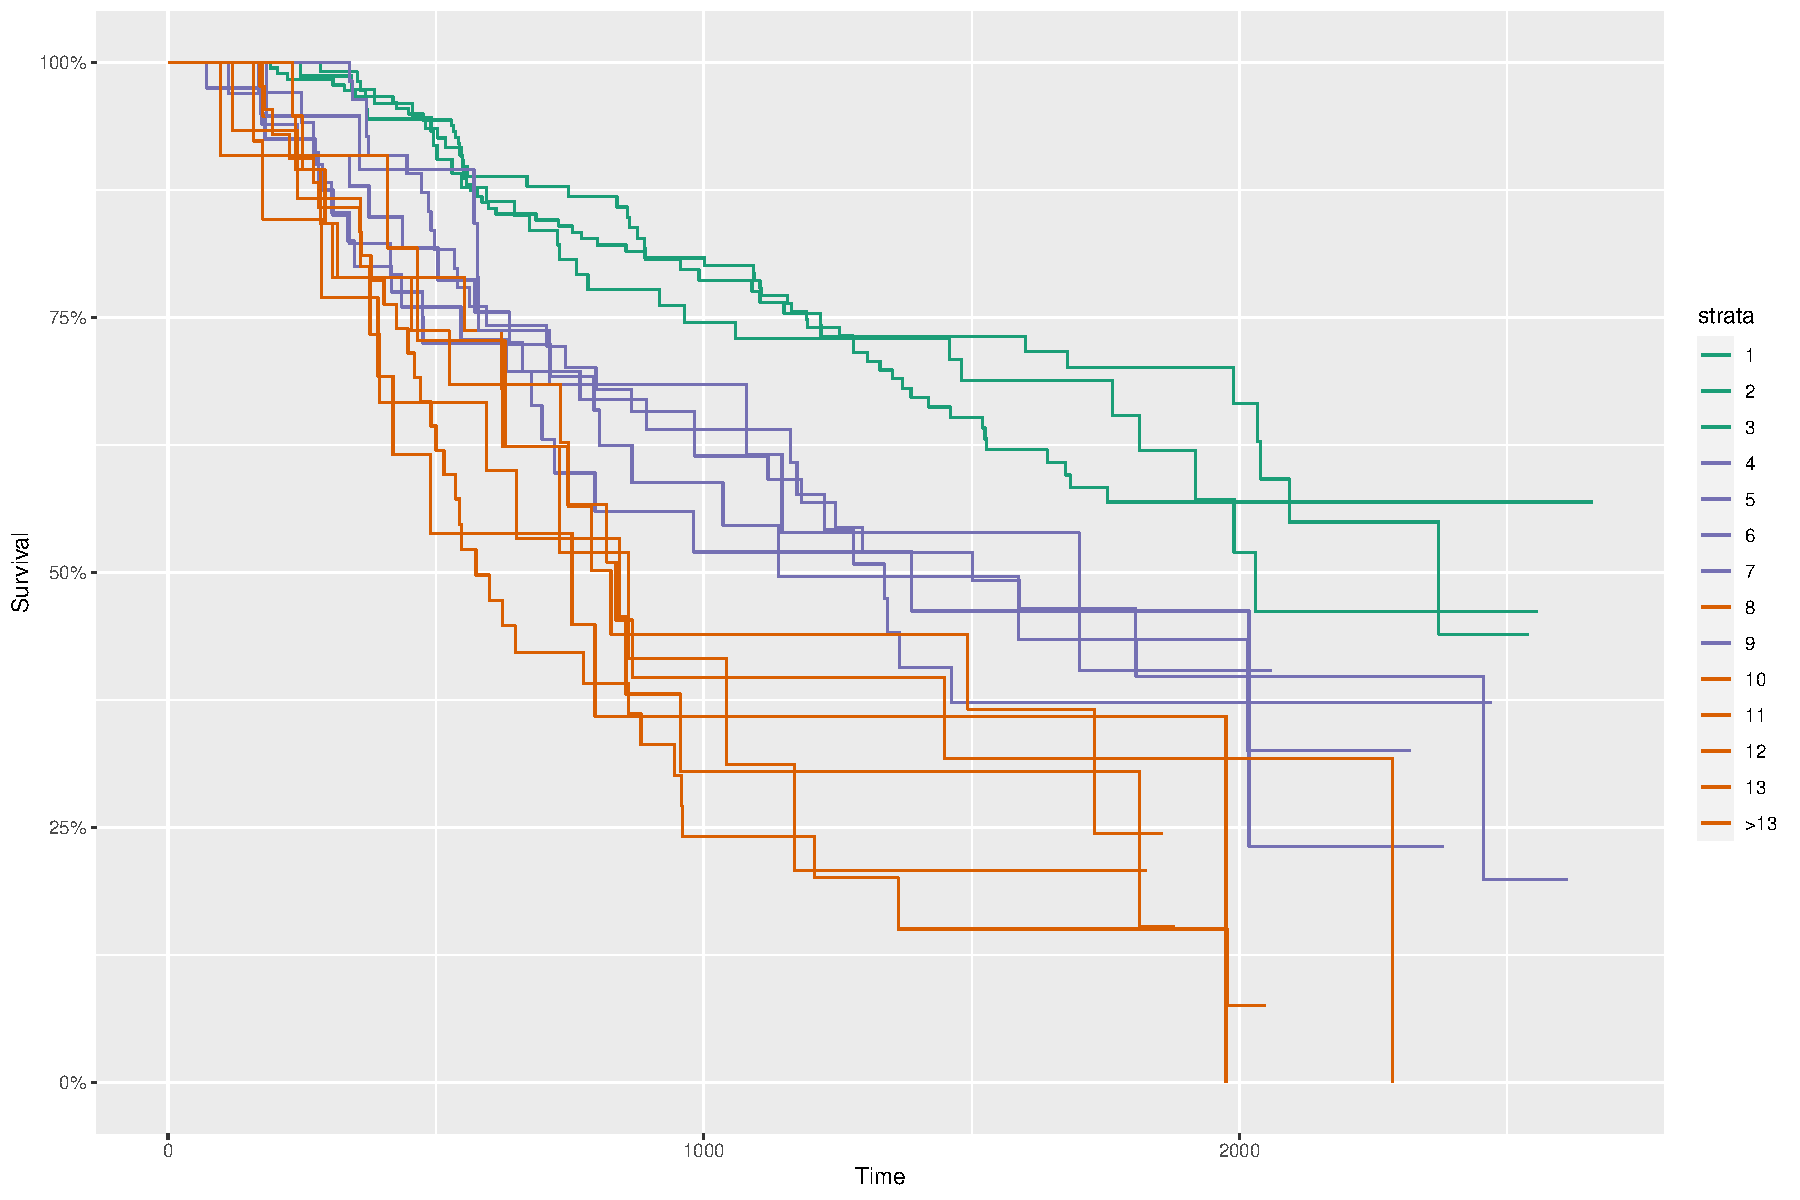
\includegraphics[width = 14cm]{breast_cancer_kmedians.pdf}
\caption{\label{noramv:gbcskmedians}
Estimated survival curves for each of the levels of the variable \code{nodes}. A specific color is assigned for each curve according to the group to which it belongs using the $K$-medians algorithm (in this case, three groups, $K$ = 3).}
\end{figure}


Equivalently, the following piece of code shows the input commands and the results obtained with the \code{algorithm = 'kmeans'}. However, the number of groups and the assignments are  different from those  obtained with the \code{'kmedians'}. Although this situation is not so common, in some real applications, it can happen.  


\begin{example}
> fit.gbcs2 <- survclustcurves(time = gbcsCS$rectime, status = gbcsCS$censrec, 
		 x = gbcsCS$nodes, nboot = 500, seed = 300716, algorithm = 'kmeans',
	         cluster = TRUE)
Checking 1 cluster... 
Checking 2 clusters... 

Finally, there are 2 clusters.


> fit.gbcs2

Call:  
survclustcurves(time = gbcsCS$rectime, status = gbcsCS$censrec, 
    x = gbcsCS$nodes, nboot = 500, algorithm = "kmeans", cluster = TRUE, 
    seed = 300716)

Clustering curves in 2 groups

Number of observations:  607
Cluster method:  kmeans
\end{example}


The corresponding plot is shown in Figure \ref{noramv:gbcskmeans}. Note that having 9 or more positive nodes seems to be related to a lower recurrence-free survival than having 9 or less, with the exception of the survival curve for those patients with 8 positive nodes, which was assigned to the group with highest recurrence probabilities.



\begin{figure}[htbp]
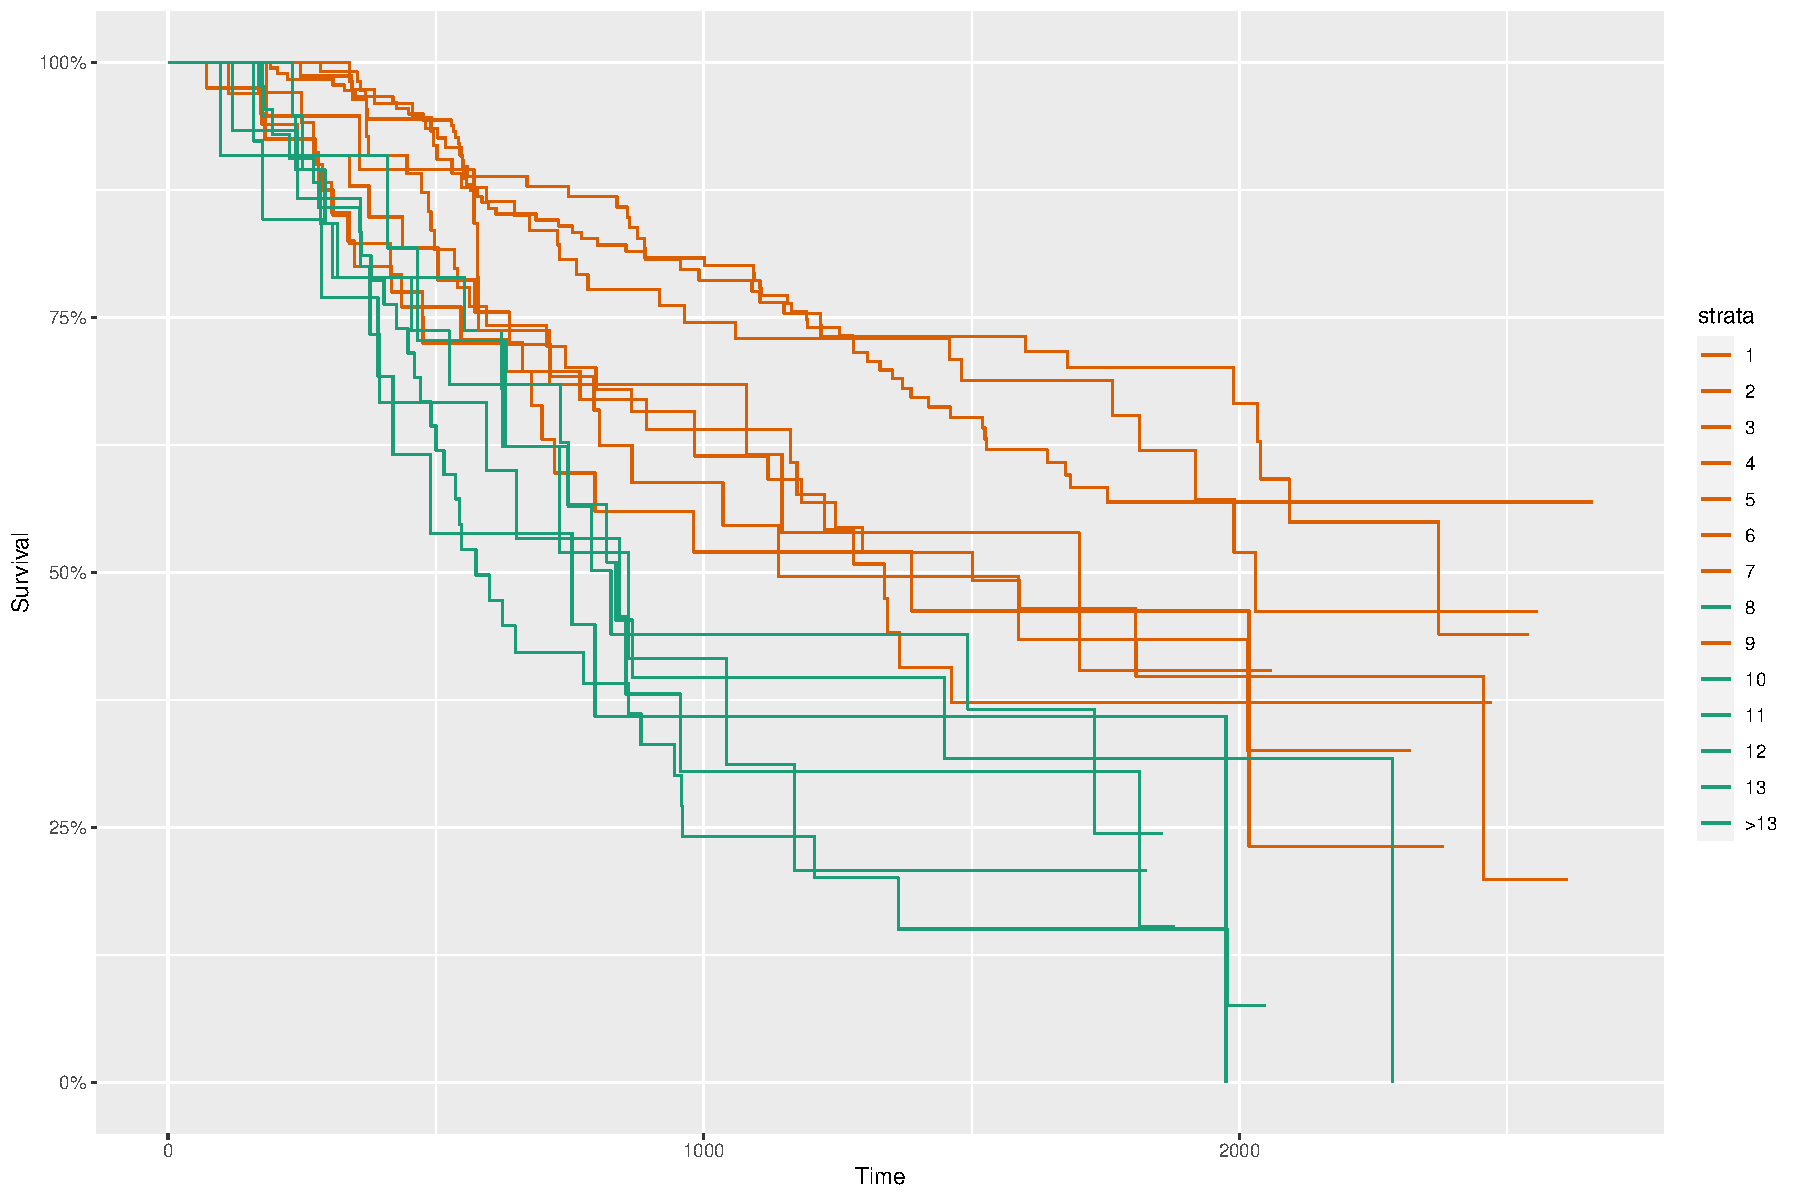
\includegraphics[width = 14cm]{breast_cancer_kmeans.pdf}
\caption{\label{noramv:gbcskmeans}
Estimated survival curves for each of the levels of the variable \code{nodes}. A specific color is assigned for each curve according to the group to which it belongs using the $K$-means algorithm (in this case, two groups, $K$ = 2).}
\end{figure}



It is important to highlight that given a fixed value of $K$, one may also be interested in determining the group to which each survival function belongs. This is possible by means of the \code{ksurvcurves} function by considering, for example, the argument \code{k = 3}.


\begin{example}
> ksurvcurves(time = gbcsCS$rectime, status = gbcsCS$censrec, x = gbcsCS$nodes, 
		    seed = 300716, algorithm = 'kmedians', k = 3)

Call:  
ksurvcurves(time = gbcsCS$rectime, status = gbcsCS$censrec, x = gbcsCS$nodes, 
    k = 3, algorithm = "kmedians", seed = 300716)

Clustering curves in 3 groups

Number of observations:  640
Cluster method:  kmedians
\end{example}

More information related to  the output above can be obtained running the \code{summary} function. 


 
\subsection{Application to Multiple Myeloma Study Data}



In this case, a study of the survival in patients with multiple myeloma (MM) cancer was conducted. 256 individuals were included from the start of the follow-up to whom were analyzed and collected 16 variables. This data set is freely available in the \pkg{survminer} package. Below, it is shown the first rows of the \code{data.frame} with columns such as treatment (\code{treatment}), life state indicator (\code{event}; censored -- 0; 1 -- dead), survival time (\code{time}, in months), among others.

\newpage
\begin{example}
> library(survminer)
> data(myeloma)
> head(myeloma[,1:5])
         molecular_group chr1q21_status treatment event  time
GSM50986      Cyclin D-1       3 copies       TT2     0 69.24
GSM50988      Cyclin D-2       2 copies       TT2     0 66.43
GSM50989           MMSET       2 copies       TT2     0 66.50
GSM50990           MMSET       3 copies       TT2     1 42.67
GSM50991             MAF           <NA>       TT2     0 65.00
GSM50992    Hyperdiploid       2 copies       TT2     0 65.20
\end{example}


In this example, it is  interesting to analyze if the survival in patients with  MM disease  is the same for  the different  molecular subgroups. If there is an effect of the  molecular subgroups on the  survival, future therapies that might exploit molecular insights should lead to an improvement in outcome for patients with these types of disease \citep{blood}. 

Below, a summary of the results of the  \code{survclustcurves} function obtained with  \code{time}, \code{event}, and \code{molecular\_group} as input variables and for both  \code{kmedians} and \code{kmeans}  algorithms are shown.

\begin{example}
> fit.mye <- survclustcurves(time = myeloma$time, status = myeloma$event, 
                      x = myeloma$molecular_group, nboot = 500, seed = 300716,
                      algorithm = 'kmedians', cluster = TRUE)
Checking 1 cluster... 
Checking 2 clusters... 

Finally, there are 2 clusters. 
> summary(fit.mye)

Call:  
survclustcurves(time = myeloma$time, status = myeloma$event, 
    x = myeloma$molecular_group, nboot = 500, algorithm = "kmedians", 
    cluster = TRUE, seed = 300716)

Clustering curves in 2 groups

Number of observations:  248
Cluster method:  kmedians 

Factor's levels:
[1] "Cyclin D-1"       "Cyclin D-2"       "Hyperdiploid"     "Low bone disease"
[5] "MAF"              "MMSET"            "Proliferation"   

Clustering factor's levels:
[1] 1 1 1 1 1 2 2

Testing procedure:
  H0   Tvalue pvalue
1  1 31.31603  0.026
2  2 14.94269  0.682

Available components:
 [1] "num_groups" "table"      "levels"     "cluster"    "centers"    "curves"    
 [7] "method"     "data"       "algorithm"  "call"       

> fit.mye2 <- survclustcurves(time = myeloma$time, status = myeloma$event, 
                      x = myeloma$molecular_group, nboot = 500, seed = 300716,
                      algorithm = 'kmeans', cluster = TRUE)
Checking 1 cluster... 
Checking 2 clusters... 

Finally, there are 2 clusters. 





> summary(fit.mye2)

Call:  
survclustcurves(time = myeloma$time, status = myeloma$event, 
    x = myeloma$molecular_group, nboot = 500, algorithm = "kmeans", 
    cluster = TRUE, seed = 300716)

Clustering curves in 2 groups

Number of observations:  248
Cluster method:  kmeans 

Factor's levels:
[1] "Cyclin D-1"       "Cyclin D-2"       "Hyperdiploid"     "Low bone disease"
[5] "MAF"              "MMSET"            "Proliferation"   

Clustering factor's levels:
[1] 1 1 1 1 1 2 2

Testing procedure:
  H0   Tvalue pvalue
1  1 4.500272  0.032
2  2 1.108812  0.730

Available components:
 [1] "num_groups" "table"      "levels"     "cluster"    "centers"    "curves"    
 [7] "method"     "data"       "algorithm"  "call"   
\end{example} 



When comparing the results obtained through the two methods (\code{kmeans}, \code{kmedians}), it is seen that the obtained number of clusters  is the same (2 groups), even the assignment of the curves to the groups. 

In particular, results obtained  reveal that MMSET level and Proliferation level are associated with a high-risk or damage on the lifetime, while  MAF, Low bone disease, Hyperdiploid, Cycline D-1, and Cycline D-2  have higher survival probabilities. This is observed in the plot shown in Figure \ref{noramv:fig2kmedians}, which can be obtained using the following input command:


\begin{example}
> autoplot(fit.mye, groups_by_color = TRUE) 
\end{example}


\begin{figure}[htbp]
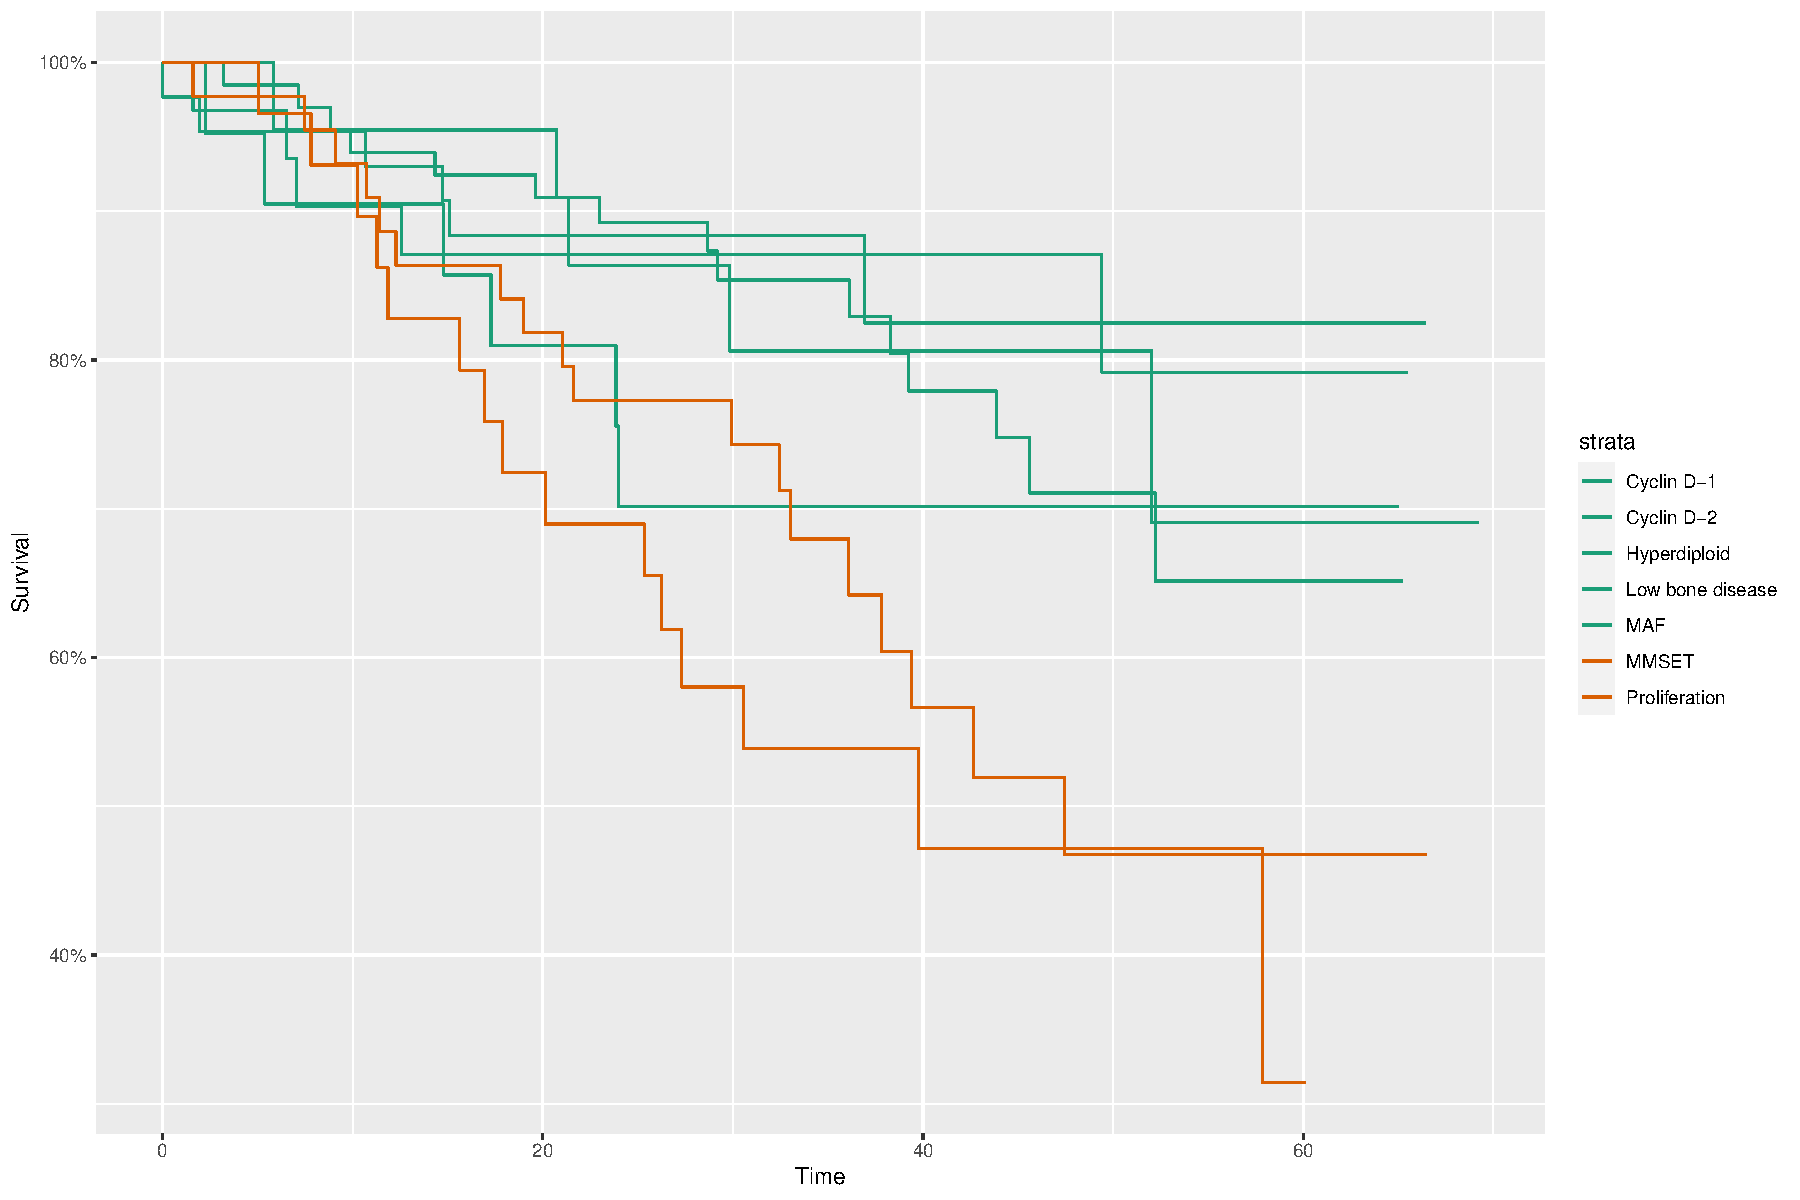
\includegraphics[width = 14cm]{myeloma_cancer_kmedians.pdf}
\caption{\label{noramv:fig2kmedians}
Estimated survival curves for each of the levels of the variable \code{molecular group}. A specific color is assigned for each curve according to the group to which it belongs using the $K$-medians algorithm, two groups, $K$ = 2.}
\end{figure}



\subsection{Application to Barnacle's Growth Study Data}

This study was conducted on the Atlantic coast of Galicia (Northwest Spain), which consists of an approximately 1000km long shoreline with extensive rocky stretches exposed to tidal surges and wave action that are settled by the \textit{Pollicipes pollicipes} (Gmelin, 1789) populations targeted for study. A total of 5000 specimens were collected from five sites of the region's Atlantic coastline and corresponded to the stretches of coast where this species is harvested: Punta do Mouro, Punta Lens, Punta de la Barca, Punta del Boy and Punta del Alba. Two biometric variables of each specimen were measured: RC (Rostro-carinal length, maximum distance across the capitulum between the ends of the rostral and carinal plates) and  DW (Dry Weight). This data set (\code{barnacle5}) is available in the \pkg{clustcurv} package. The idea of this study is to know the relation between RC and DW variables along the coast, i.e., to analyze if  the barnacle's growth is similar in all locations  or by contrast, if it is possible to detect geographical differentiation in growth.
A sample of the dataset is shown as follow:

\begin{example}
> data("barnacle5")
> head(barnacle5)
    DW   RC    F
1 0.52 12.0 laxe
2 1.46 18.9 laxe
3 0.05  6.4 laxe
4 0.17  9.4 laxe
5 0.05  6.2 laxe
6 0.41 12.2 laxe
\end{example}
 
\newpage

For each location (\code{F}), nonparametric regression curves were estimated to modeling the dependence between RC and DW. In order to determine groups, we used the proposed methodology in Subsection \ref{nmvillanueva:regalgorithm}. Through executing the next piece of code, the following results can be obtained: one estimated  curve was attributed to the first group (Punta Lens), two estimated curves were assigned to  group 2 (Punta de la Barca and Punta del Boy), and the other two belong to  group 3 (Laxe do Mouro and Punta del Alba) (Figure \ref{noramv:barnacle5kmeans}). In this example, the \code{regclustcurves} function was used with \code{algorithm = 'kmeans'}  and the input variables $y, x, z$.

\begin{example}
> fit.bar <- regclustcurves(y = barnacle5$DW, x = barnacle5$RC, z = barnacle5$F,
               nboot = 500, seed = 300716, algorithm = 'kmeans', cluster = TRUE)
               
Checking 1 cluster... 
Checking 2 clusters... 
Checking 3 clusters... 

Finally, there are 3 clusters. 

> summary(fit.bar)

Call:  
regclustcurves(y = barnacle5$DW, x = barnacle5$RC, z = barnacle5$F, 
    nboot = 500, algorithm = "kmeans", cluster = TRUE, seed = 300716)

Clustering curves in 3 groups

Number of observations:  5000
Cluster method:  kmeans 

Factor's levels:
[1] "laxe"  "lens"  "barca" "boy"   "alba" 

Clustering factor's levels:
[1] 2 1 3 3 2


Testing procedure:
  H0     Tvalue pvalue
1  1 0.94353014  0.000
2  2 0.15463483  0.034
3  3 0.02348982  0.422

Available components:
 [1] "num_groups" "table"      "levels"     "cluster"    "centers"    "curves"    
 [7] "method"     "data"       "algorithm"  "call"
\end{example}





As can be seen, Figure \ref{noramv:barnacle5kmeans} obtained using the following input command. The specimens from Punta de la Barca and Punta del Boy have similar morphology, wide and short. This is due to these zones present similar oceanographic characteristic, such as exposed rocky shore to waves and highly articulated. Unlike, the barnacles collected from Laxe do Moure and Punta del Alba are narrow and long because they are less exposed locations. Finally, Punta Lens is an intermediate coast, alternating sections of steep coast with large sand. 



\begin{example}
> autoplot(fit.bar, groups_by_color = TRUE)
\end{example}





\begin{figure}[htbp]
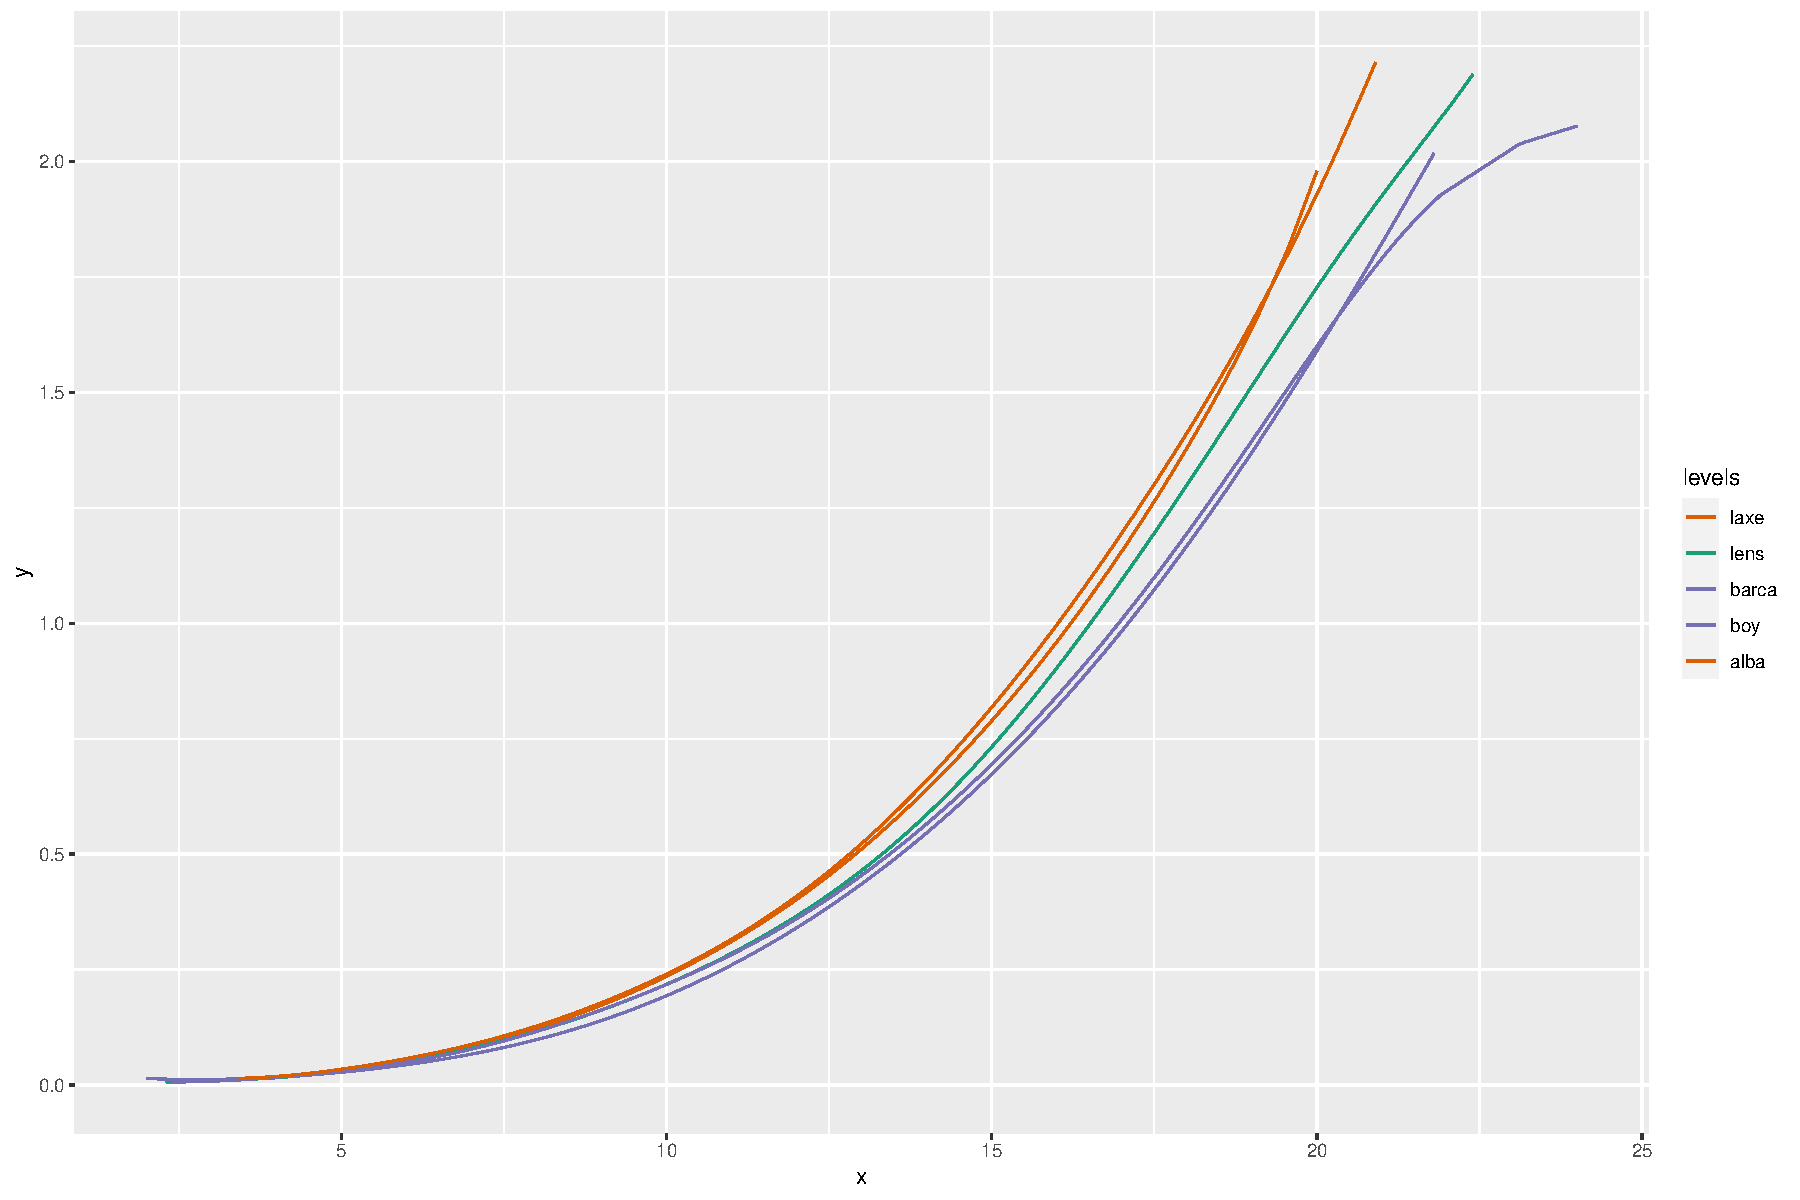
\includegraphics[width = 14cm]{barnacle5_kmeans.pdf}
\caption{\label{noramv:barnacle5kmeans}
Estimated regression curves for each of the levels of the factor. A specific color is assigned for each curve according to the group to which it belongs using the $K$-means algorithm (in this case, three groups, $K$ = 3).}
\end{figure}





\subsection{Application to simulated data}

Finally, this subsection reports the capabilities of the \pkg{clustcurv} package in a more complicated simulated scenario. We consider the regression models given in (\ref{noramv:eq1}) for $j=1, \ldots, 30$, with

\begin{equation}
m_j(X_j)=\left \{ {
\begin {tabular} {lcc}
$X_j + 1 $ \hspace{1.90cm} {\text if} \quad $j \le 5 $\\
$X_j^2 + 1$ \hspace{1.90cm} {\text if} \quad $5 < j \le 10 $\\
$2 \hspace{0.10cm} {\rm sin} \hspace{0.05cm}(2 \hspace{0.10cm}X_j)$ \hspace{1.22cm} {\text if} \quad $10 < j \le 15 $\\
$2 \hspace{0.10cm} {\rm sin}\hspace{0.05cm}(X_j)$ \hspace{1.45cm} {\text if} \quad $15 < j \le 20 $\\
$2 \hspace{0.10cm} {\rm sin} \hspace{0.05cm}(X_j) + a \hspace{0.10cm} \mathrm{e}^{X_j}$ \hspace{0.35cm} {\text if} \quad $20 < j \le 25 $\\
$1$  \hspace{2.65cm} {\text if} \quad $j > 25 $,\\
\end {tabular}
}\right.
\label{noramv:eq2}
\end{equation}

\noindent where $a$ is a real constant, $X_j$ is the explanatory covariate drawn from a   uniform distribution $[-2,2]$, and  $\varepsilon_j$ is the error distributed in accordance to a $N(0, \sigma_j(x))$. We have considered the heteroscedastic scenario where  $\sigma_j(x)=0.5+0.05m_j(x) \cdot N(0, 1.5)$.

We explore the methodology considering the null hypothesis $H_0(5)$ of assignment of the $m_j$ curves  into five groups ($K= 5$). To show the performance of our procedure, two values were considered for $a$,  0 and 0.4. It should be noted that the value  $a=0$ corresponds to the null hypothesis, while if $a=0.4$ the number of groups is six. Particularly, we have defined an unbalanced scenario with unequal sample sizes for each $j$ curve, particularly, $(n_1, n_2, \ldots, n_J) \sim$ Multinomial$(n;  p_1, p_2, \ldots, p_J)$  being $p_j = p_j^\ast /\sum_{j=1}^{J} p_j^\ast$, with  $p_j^\ast$ randomly drawn from  $\{1, 1.5, 2, 2.5, 3\}$ and $n = 5000$. Note that we propose this procedure for generating the  $n_j$ in order to obtain a completely unbalanced study.



The code for the generation of this dataset with $a=0$ can be found below:

\begin{example}
> m <- function(x, j) {
   y <- numeric(length(x))
   y[j <= 5] <- x[j <= 5] + 1
   y[j > 5 & j <= 10] <- x[j > 5 & j <= 10] ^ 2 + 1
   y[j > 10 & j <= 15] <- 2 * sin(2 * x[j > 10 & j <= 15]) #- 4
   y[j > 15 & j <= 20] <- 2 * sin(x[j > 15 & j <= 20])
   y[j > 20 & j <= 25] <- 2 * sin(x[j > 20 & j <= 25]) + a * exp(x[j > 20 & j <= 25])
   y[j > 25] <- 1
   return(y)
 }

> seed <- 300716
> set.seed(seed)
> n <- 5000
> a <- 0.0
> x <- runif(n, -2, 2)
> prob <- sample(c(1, 1.5, 2, 2.5, 3), 30, replace = TRUE)
> prob <- prob/sum(prob)
> f <- sample(1:30, n, replace = TRUE, prob = prob)
> N <- length(unique(f))
> error <- rnorm(n,0,1.5)
> y <- m(x, f) + (0.5 + 0.05 * m(x, f)) * error 
> data <- data.frame(x, y, f)
\end{example}

In order to determine groups of the generated curves, the user has to execute the  next piece of code. As expected, when $a=0$, the number of groups selected is five. 


\begin{example}
> fit.sim <- regclustcurves(x = data$x, y = data$y,  z = data$f, nboot = 500, 
                     algorithm = 'kmedians', cluster = TRUE, seed = 300716)
Checking 1 cluster... 
Checking 2 clusters... 
Checking 3 clusters... 
Checking 4 clusters... 
Checking 5 clusters... 

Finally, there are 5 clusters. 
> fit.sim

Call:  
regclustcurves(y = data$y, x = data$x, z = data$f, nboot = 500, 
    algorithm = "kmedians", cluster = TRUE, seed = 300716)

Clustering curves in 5 groups

Number of observations:  5000
Cluster method:  kmedians
> autoplot(fit.sim, groups_by_colour = TRUE, centers = TRUE)
\end{example}

Additionally, for different values of $a$ (a > 0), our procedure should determine 6 groups. For instance, for $a = 0.4$, it selects the true number of groups ($K=6$) typing the commands below:  


\begin{example}
> seed <- 300716
> set.seed(seed)
> n <- 5000
> a <- 0.4
> x <- runif(n, -2, 2)
> prob <- sample(c(1, 1.5, 2, 2.5, 3), 30, replace = TRUE)
> prob <- prob/sum(prob)
> f <- sample(1:30, n, replace = TRUE, prob = prob)
> N <- length(unique(f))
> error <- rnorm(n,0,1.5)
> y <- m(x, f) + (0.5 + 0.05 * m(x, f)) * error
> data2 <- data.frame(x, y, f)
> fit.sim2 <- regclustcurves(x = data2$x, y = data2$y,  nboot = 500, seed = 300716,
                         z = data$f, algorithm = 'kmedians', cluster = TRUE)		       
Checking 1 cluster... 
Checking 2 clusters... 
Checking 3 clusters... 
Checking 4 clusters... 
Checking 5 clusters... 
Checking 6 clusters... 

Finally, there are 6 clusters. 
> fit.sim2

Call:  
regclustcurves(y = data2$y, x = data2$x, z = data$f, nboot = 500, 
    algorithm = "kmedians", cluster = TRUE, seed = 300716)

Clustering curves in 6 groups

Number of observations:  5000
Cluster method:  kmedians
> autoplot(fit.sim2, groups_by_colour = TRUE, centers = TRUE)
\end{example}



Figures \ref{noramv:sim_5kmeans} and  \ref{noramv:sim_6kmeans} show the results  with the simulated data with $a=0$ and  $a=0.4$, respectively. In this situation, the true number of groups is equal to 5 and 6.  As can be appreciated, our method seems to perform reasonably well for both values of $a$. For $a=0$, the null hypothesis $H_0(5)$ is accepted, curves assigned to each group are plotted with the same color. In the case of $a=0.4$, the null hypothesis $H_0(6)$ is accepted.  Therefore, there are 6 groups of regression curves.  Note that in both plots, the centroids are colored in black because in the \code{autoplot} function, the argument  \code{centers = TRUE}. 




\begin{figure}[htbp]
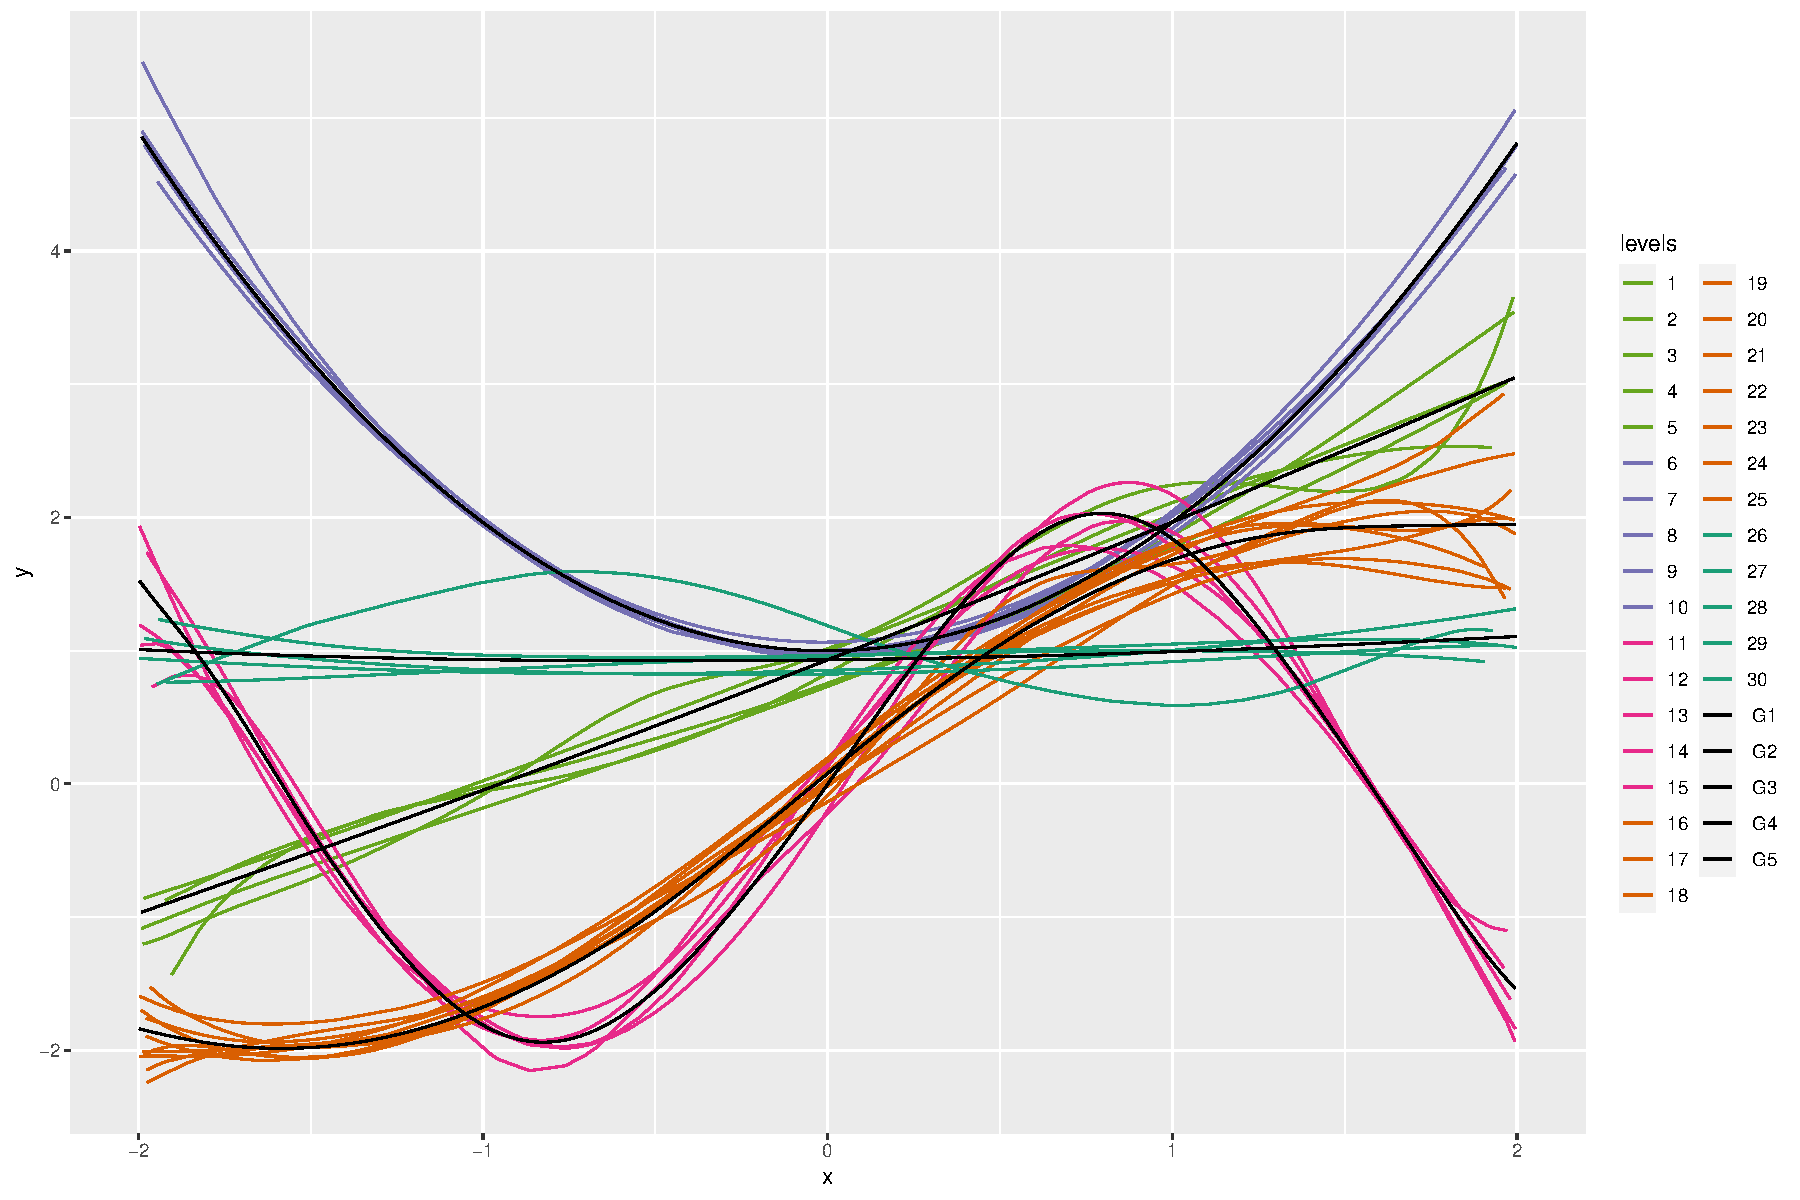
\includegraphics[width = 14cm]{sim_5kmeans.pdf}
\caption{\label{noramv:sim_5kmeans}
Estimated regression curves for each of the levels of the variable \code{f} with $a=0$. A specific color is assigned for each curve according to the group to which it belongs using the $K$-means algorithm (in this case, five groups, $K$ = 5). Black curves are the centroids of each group.}
\end{figure}


\begin{figure}[htbp]
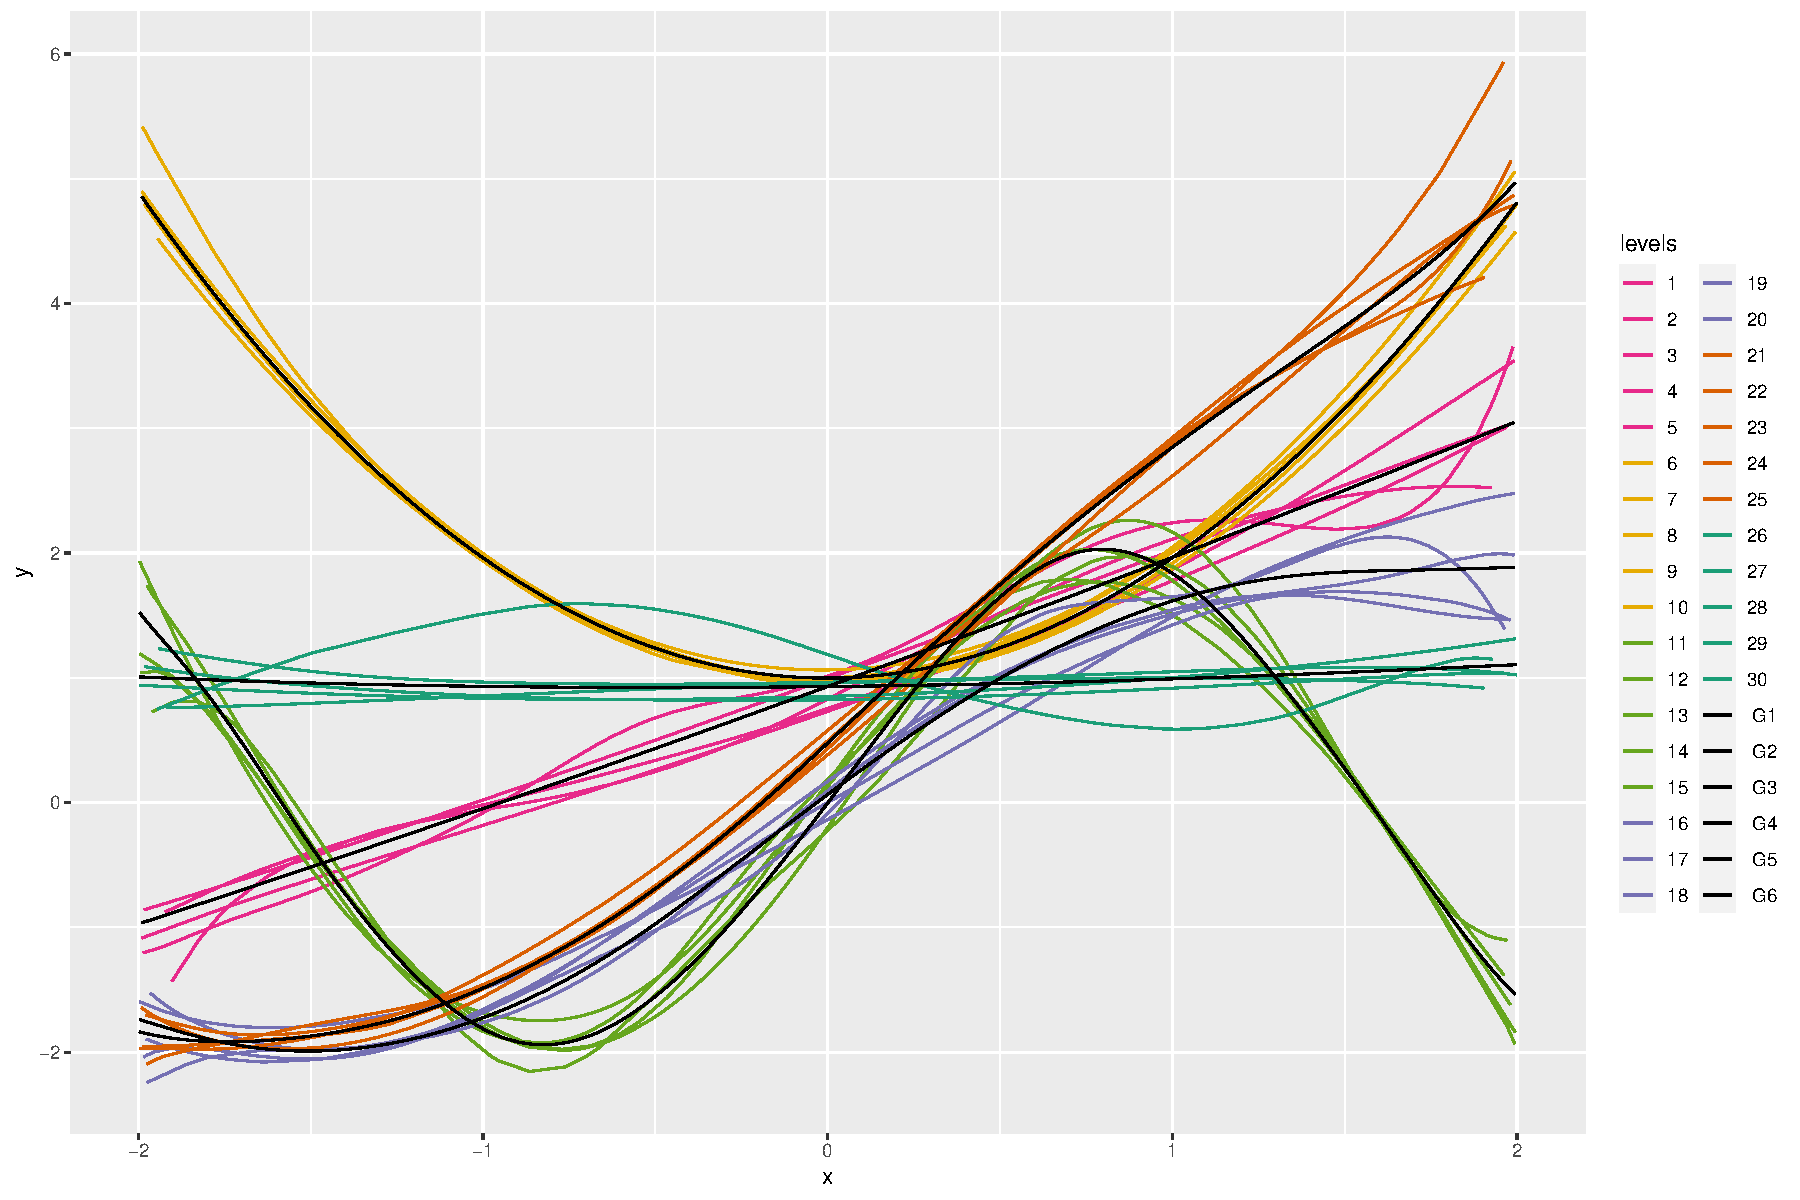
\includegraphics[width = 14cm]{sim_6kmeans.pdf}
\caption{\label{noramv:sim_6kmeans}
 Estimated regression curves for each of the levels of the variable \code{f} with $a=0.4$. A specific color is assigned for each curve according to the group to which it belongs using the $K$-means algorithm (in this case, six groups, $K$ = 6). Black curves are the centroids of each group.}
\end{figure}


\section*{Conclusion and further extensions of the R package}


This paper discussed the implementation of some methods developed for determining groups of multiple nonparametric curves in the R package \pkg{clustcurv}. In particular, the methods proposed are focused on the framework of regression analysis and in the framework of survival analysis. In the context of survival analysis, we restrict ourselves to survival curves. Hopefully, future versions of the package will extend the methodology to determine groups in risk functions, cumulative hazard curves, or density functions. The current version of the package implements two optimization algorithms, the well-known $K$-means and $K$-medians. It can be interesting to let the user choose far from those, such as Means-Shift or $K$-medoids algorithms.




\section*{Acknowledgements}

%The authors acknowledge financial support by Spanish Ministry of Economy and Competitiveness (MINECO) through project MTM2017-89422-P and MTM2017-82379-R and acronym AFTERAM, both funded by (funded by (AEI/FEDER, UE). We also acknowledge the financial support provided by the SiDOR (Statistical Inference, Decision and Operations Research, University of Vigo) Spain group through the grant Competitive Reference Group, 2016/2019 (ED431C 2016/040) funded by the Conseller\'ia de Cultura, Educaci\'on e Ordenaci\'on Universitaria, Xunta de Galicia, Spain. Finally, support from the Xunta de Galicia and the European Union (FEDER) through Singular Research Center (2016-2019 ED431G/02 and 2019-2022 ED431G/06), is gratefully acknowledged.  Thanks to the Associate Editor and the referee for comments and suggestions that have improved this paper. 
The authors acknowledge financial support by the Spanish Ministry of Economy and Competitiveness (MINECO) through project MTM2017-89422-P and MTM2017-82379-R (funded by (AEI/FEDER, UE). Thanks to the Associate Editor and the referee for comments and suggestions that have improved this paper.
\break
\bibliography{villanueva_sestelo_meira_roca}

\address{Nora M. Villanueva\\
Department of Statistics and OR,\\
SiDOR research group \& CINBIO\\
University of Vigo, Spain\\
ORCiD: 0000-0001-8085-2745\\
\url{http://noramvillanueva.github.io}\\
\email{nmvillanueva@uvigo.es}}


\address{Marta Sestelo\\
Department of Statistics and OR,\\
SiDOR research group \& CINBIO\\
University of Vigo, Spain\\
ORCiD: 0000-0003-4284-6509\\
\url{http://sestelo.github.io}\\
\email{sestelo@uvigo.es}}

\newpage

\address{Lu\'is Meira-Machado\\
Department of Mathematics\\
Centre of Mathematics\\
University of Minho, Portugal\\
\email{lmachado@math.uminho.pt}}

\address{Javier Roca-Pardi\~nas\\
Department of Statistics and OR,\\
SiDOR research group \& CINBIO\\
University of Vigo, Spain\\
\email{roca@uvigo.es}}
\end{article}

\end{document}
